
\section{Container Networking with \wnet}
\wnet\ is an open source project\footnote{\url{www.github.com/weaveworks/weave}} which is developed by a global team, mostly employed by the London-based software company \emph{Weaveworks}.\footnote{\url{www.weave.works}} The purpose of \wnet\ is to provide advanced overlay networking capabilities for \docker\ containers. As such, is designed to make up for the shortcomings of \docker 's built-in overlay networks, and more specifically, their lack of encryption and multicast support. By means of \weave\ overlay networks, dispersed containers deployed on physically isolated hosts around the world, may communicate as if they were connected via LAN. From a containerized applications' viewpoint, it does not matter whether its peers are located on the same host or within a data center on the other side of the world.

\subsection{Functioning}
\wnet\ is implemented as client software which is installed on each machine that partakes in the overlay. The software can be started using a single command, and in the following, all containers launched on that host will automatically connected to the overlay network. This is achieved by means of a \emph{\docker\ API proxy}. The proxy sits between \docker 's command-line client and the \docker\ daemon and intercepts all communication between the two. When the \docker\ engine is instructed to start a container, the proxy takes all precautions needed to enable overlay networking for that container. Once the connection is established, all container traffic is routed through three dedicated network channels: one TCP connection to exchange meta data about the network, and two UDP channels for duplex data exchange.

\begin{figure}[htpb]
  \centering
  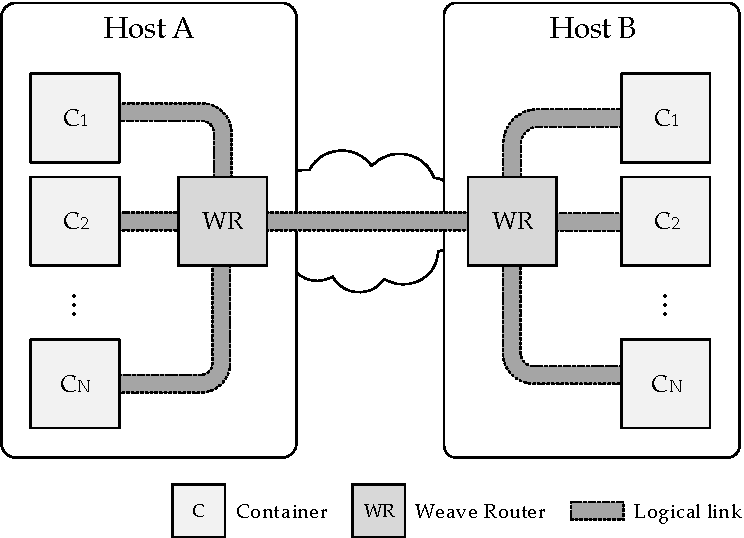
\includegraphics[width=0.7\textwidth]{figures/weave.pdf}
  \caption[An example of containers connected via \wnet\ overlay network]{A number of dispersed containers connected by a \wnet\ overlay network}\label{fig:weavescheme}
\end{figure}

When the \weave\ software is started, a central component of \wnet , the \emph{\weave\ router} is launched (\cf \Cref{fig:weavescheme}). Similar to a hardware router, the \weave\ router is responsible for the forwarding and routing of data packets to their appropriate receivers. \weave\ routers can be seen as gateways through which all containers participating in a \weave\ network are connected. To facilitate routing on the data plane, a custom UDP encapsulation protocol, called \emph{sleeve}, was devised. A \weave\ router in itself is an containerized application running at all times, in the same way a daemon would. There is one of such router containers running on every host in a \weave -enabled infrastructure.

The \weave\ router is a user space process. As such, a context switch is needed every time it is tasked to process a packet. This comes with a substantial performance overhead. Hence, as a faster alternative, the so-called \emph{fast datapath} mode was added. In this mode, packets are processed by the Linux kernel instead of by the \weave\ router. This way, the context switch into user space is omitted. \wnet\ leverages the Linux kernel's Open vSwitch datapath module (\cf \Cref{sec:overlays}) to achieve this behavior. Open vSwitch can be used to create a virtual, software-based network switch. That way, the kernel can be instructed to process packets in a certain way. For instance, the kernel can be commanded to add a VXLAN header to each packet, thereby achieving the same result as the \weave\ router, but faster. However, fast datapath mode can only be used when the underlying infrastructure allows it. The Internet is a particular example of a network where fast datapath communication is hard to achieve.


\subsection{Topology Management}
\weave 's topology management is self-governing and self-healing. Peers continually exchange topology information and monitor the state of the network. Whenever peers lose connectivity, they continuously try to re-establish the connection until it is restored. All participating peers know the topology of the entire network. For this, \wnet\ employs a sophisticated discovery and topology management mechanism by which changes in the network topology are rapidly propagated within the network. The topology management protocol is based on a spanning-tree broadcast mechanism known from hardware switches. To further ensure that all peers have an up-to-date neighbor list at all times, \wnet\ additionally employs a custom neighbor gossiping protocol by which each peer sends update messages to a random subset of their neighbors. Updates of the network's topology are performed periodically as well as when certain events occur, such as when a node joins or leaves the network.

In order to add a new host to the overlay, the \weave\ software needs to be started on that host, referencing at least one other host in the network by its IP address. The information that a new host was added is then propagated to the other hosts in the overlay. After a short period, all hosts know that the new host was added and that a path to that host exists.

\subsection{Encryption}
As mentioned earlier, a salient feature of \wnet\ is the ability to encrypt all traffic within the overlay network.\footnote{Encryption applies end-to-end between \weave\ routers. For containers hosted on the same machine, communication is not encrypted.} This is especially important for networks that span over insecure underlays, such as the Internet. To set up encryption, a shared secret (password) needs to be provided when the \weave\ router is launched. The shared secret must therefore be present on all participating hosts. From the password, salted, ephemeral session keys are generated which are then used to encrypt the network packets' payload. For each connection between any two \weave Routers, one unique session key exists.

The way encryption is applied differs depending on the forwarding mode used (sleeve or fast datapath). In fast datapath mode, a IPsec-based protocol is used, whereby each packet is wrapped in an encapsulated security payload (ESP). Because each packet in this mode is processed by the Linux kernel, encryption is applied by means of the standard Linux Kernel Crypto API which is thoroughly tested, and generally considered secure. For sleeve mode, a custom encryption algorithm based on TLS\footnote{``Transport Layer Security''} is used. As with fast datapath encryption, sleeve mode encryption utilizes shared, ephemeral session keys for each connection.

\begin{figure}[htpb]
  \centering
  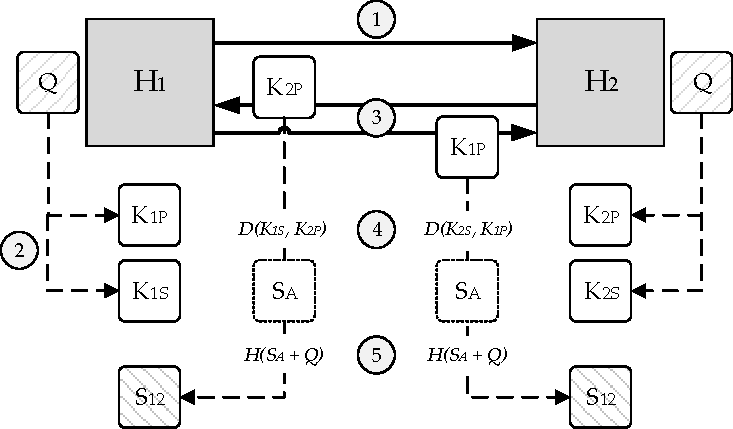
\includegraphics[width=0.6\textwidth]{figures/weave-encryption.pdf}
  \caption[\weave 's key exchange protocol]{\wnet 's key exchange protocol in sleeve mode}\label{fig:weaveencryption}
\end{figure}
\Cref{fig:weaveencryption} depicts the method used for generating and distributing session keys. In the image, two hosts ($H_1$, $H_2$) are to establish an encrypted connection. First, $H_1$ initiates the key exchange by sending a handshake message to $H_2$ \circled{1}. Then, both hosts generate their own, individual key pairs so that each host has a public key and a private key \circled{2}. The key pair for $H_1$ is $(K_{1P}, K_{1S})$ and the key pair for $H_2$ is $(K_{2P}, K_{2S})$. Once that is done, both hosts exchange their respective public keys, $K_{1P}$, and $K_{2P}$ \circled{3}. Using the peer's public key and their own private key, both hosts derive an auxiliary shared key, $S_A$, by means of Diffie--Hellman key exchange \cite{bresson2001provably}: $D(K_{1S},K_{2P})$ \circled{4}. Finally, the actual shared key can be generated. For this, both hosts append the password ($P$) to $S_A$ to provide authenticity. In order to bring the key to the desired length of 256 bit, the compounded key is additionally hashed via SHA256: $H(S_A, P)$ \circled{5}. The end result of this procedure is the final shared key, $S_{12}$, which is then used to encrypt the traffic between the two hosts.
%
%
%
%
%
%
%
%
%
%
%
%
%
%
%
%
%
%
%
%
